\documentclass{article}
\usepackage{latexsym}
\usepackage{amsmath}
\usepackage{algorithm}
\usepackage[noend]{algpseudocode}
% \usepackage{algorithmic}
% \usepackage{algorithmicx}
% \usepackage[]{algorithm2e}
\usepackage{hyperref}
\usepackage{listings} 
\usepackage{xcolor}
\usepackage{graphicx}
\usepackage{subfigure}

\usepackage[top=1in, bottom=1in, left=1.25in, right=1.25in]{geometry}

% \renewcommand{\thesubsection}{\Alph{subsection}}
\title{CSE 5243 Homework 5: Clustering}
\author{Yiran Cao(cao.805)}
\date{}
\begin{document}
\maketitle
\section{Design and Implementation}
	\subsection{Dataset Inspection and Data Preprocessing}
	Given the datasets, the first thing to do is checking for missing values and doing some exploratory data analysis to see if there is any necessity for data preprocessing.

	Fortunately, the three datasets, 2 two-dimensional datasets and the wine dataset, are composed of of numeric attributes and with no missing values.

	For the two dimensional datasets, since the two attributes of each data point can be regarded as a position vector, indicating the position of that point on a 2D plane, I did not do any transformation on these attributes. For the wine dataset, however, the attributes mean differently and probably have different scales, so I standardized each attribute of the wine dataset before clustering.

	\subsection{Clustering Function}
	The main functionality of this project is implemented in the clustering function, which takes two parameters, the dataset and the number of clusters. The following pseudo-code briefly explains how this function works.

	\begin{algorithm}
	\caption{Clustering}\label{alg:cluster}
		\begin{algorithmic}
		\Procedure{Clustering}{dataset, k}
			\State Initialization:
			\State $centroids \gets $ randomly select $k$ points from dataset
			\While{$dist > threshold $ and $iter < maxIter$}
				\For{each centroid}
					\State assign points that's nearest to it to its cluster
				\EndFor
				\For{each cluster}
					\State assign a new centroid, which is the mean of all points in this cluster
				\EndFor
				\State $dist \gets $ distance vector between the old and new centroids
				\State $iter \gets iter + 1$
			\EndWhile
		\EndProcedure
		\end{algorithmic}
	\end{algorithm}

	The clustering function initially assigns $k$ random points as centroids, then keeps upating the centroids until the old and new centroids are close enough (distance less than a small threshold), or the maximum number of iterations is reached.

	I apply this function to the two-dimensional datasets and also the wine dataset, with additional standardization on the wine dataset.

\section{Results and Analysis on the Two-Dimensional Dataset}
	\subsection{Dataset 1 -- Two-Dimensional Data with 2 Clusters}
		\subsubsection{Results}
		The clustering algorithm works well on dataset1, which is a two-dimensional dataset with two true clusters. With k=2, the k-means algorithm I implemented made 2 errors over the total number of 300 records.

		The scatter plots, Figure \ref{fig:easy-cluster} and Figure \ref{fig:easy-error}, demonstrate the clustering results and the comparison with true clusters.

		Figure \ref{fig:easy-cluster} shows the clustering result by the clustering algorithm I implemented compared with true clusters. . Figure \ref{fig:easy-error} makes the comparison, where the crosses are the misclustered points.

		\begin{figure}[H]
		\centering
		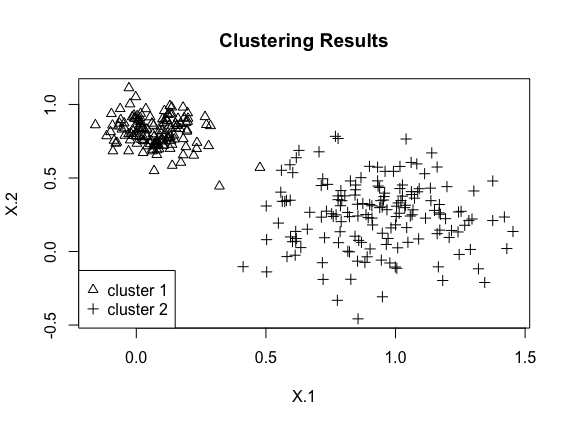
\includegraphics[width = 0.4\textwidth]{easy_cluster.png}
		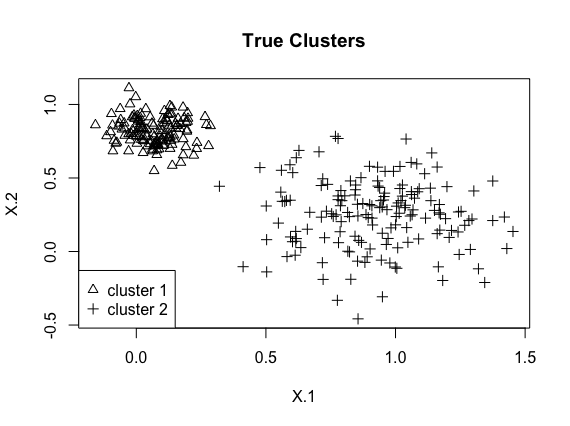
\includegraphics[width = 0.4\textwidth]{easy_true_cluster.png}
		\caption{Clustering Results \& True Clusters}
		\label{fig:easy-cluster}
		\end{figure}

		\begin{figure}[H]
		\centering
		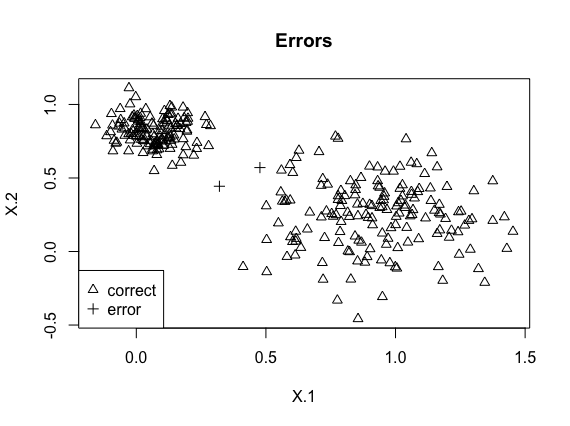
\includegraphics[width = 0.6\textwidth]{easy_errors.png}
		\caption{Clustering Errors}
		\label{fig:easy-error}
		\end{figure}

		Table \ref{tbl:cross-easy} gives an cross tabulation matrix comparing the actual and assigned clusters, from which we can see that only 2 points in true cluster 2 are misclustered into cluster 1 by the algorithm. 

		\begin{table}[H]
		\centering
			\begin{tabular}{|c||c|c|}
			\hline
			 & true cluster 1 & true cluster 2 \\
			 \hline
			 \hline
			 cluster 1 & 138 & 2 \\
			 \hline
			 cluster 2 & 0 & 160 \\
			 \hline
			\end{tabular}
			\caption{Cross Tabulation Matrix}
			\label{tbl:cross-easy}
		\end{table}

		\subsubsection{Cluster Validation}
			I calculated the SSE and SSB for both true clusters and the clusters got from the algorithm. Results are shown in Table \ref{tbl:sse-easy} and Table \ref{tbl:ssb-easy}.

			\begin{table}[H]
			\centering
				\begin{tabular}{|c|c|c|}
					\hline
					& true cluster & ``predicted'' cluster \\ 
					\hline
					1 & 2.36 & 2.78 \\
					\hline
					2 & 17 & 16.3 \\
					\hline
					overall & 13.6943 & 19.35819 \\
					\hline
				\end{tabular}
				\caption{SSE for True and ``Predicted'' Clusters}
				\label{tbl:sse-easy}
			\end{table}
			\begin{table}[H]
			\centering
				\begin{tabular}{|c|c|c|}
					\hline
					& true cluster & ``predicted'' cluster \\ 
					\hline
					SSB & 77.76 & 78.08 \\ 
					\hline
				\end{tabular}
				\caption{SSB for True and ``Predicted'' Clusters}
				\label{tbl:ssb-easy}
			\end{table}
	\subsection{Dataset 2 -- Two-Dimensional Data with 4 Clusters}
		\subsubsection{Results}
		For dataset2, the ture clusters are not so well-seperated as dataset1, with overlaps between clusters. 

		The scatter plots, Figure \ref{fig:hard-cluster} and Figure \ref{fig:hard-error}, demonstrate the clustering results and the comparison with true clusters.

		Figure \ref{fig:hard-cluster} shows the clustering result by the clustering algorithm I implemented compared to the true clusters.  Figure \ref{fig:hard-error} makes the comparison, where the crosses are the misclustered points.

		\begin{figure}[H]
		\centering
		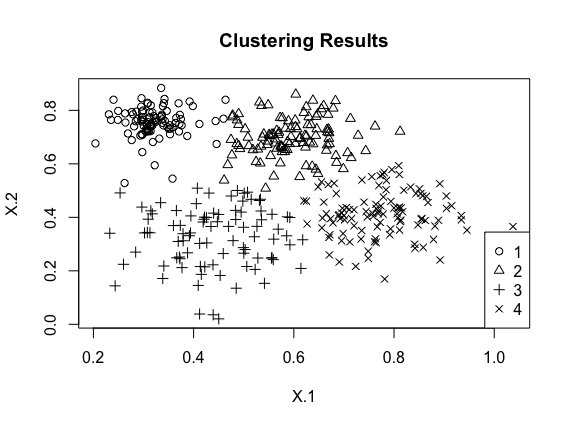
\includegraphics[width = 0.4\textwidth]{hard-cluster.png}
		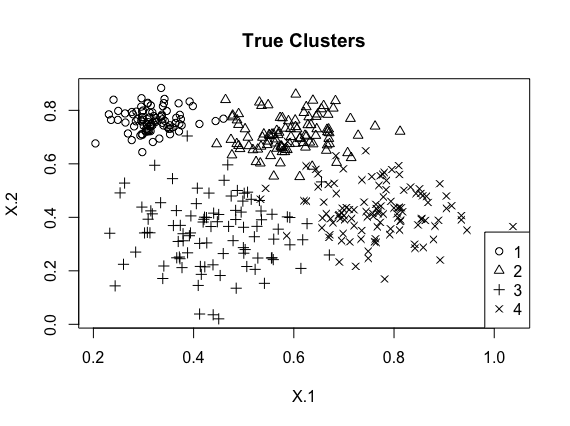
\includegraphics[width = 0.4\textwidth]{hard-true-cluster.png}
		\caption{Clustering Results}
		\label{fig:hard-cluster}
		\end{figure}
		\begin{figure}[H]
		\centering
		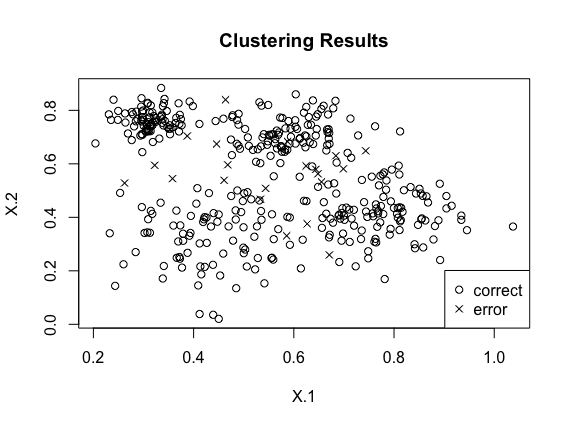
\includegraphics[width = 0.6\textwidth]{hard-error.png}
		\caption{Clustering Errors}
		\label{fig:hard-error}
		\end{figure}

		Table \ref{tbl:cross-hard} gives an cross tabulation matrix comparing the actual and assigned clusters. The numbers on the diagonal are points which are correctly clustered, while others are error points. For dataset2, the algorithm made 21 mistakes in total.

		\begin{table}[H]
		\centering
			\begin{tabular}{|c|c|c|c|c|}
			\hline
			 & true cluster 1 & true cluster 2 & true cluster 3 & true cluster 4\\
			 \hline
			 \hline
			 cluster 1 & 89  & 2 &  4 &  0 \\
			 \hline
			 cluster 2 & 0 & 98 &  2  & 8 \\
			 \hline
			 cluster 3 & 0 &  0 & 88  & 2 \\
			 \hline
			 cluster 4 & 0 &  0  & 3& 104 \\
			 \hline
			\end{tabular}
			\caption{Cross Tabulation Matrix}
			\label{tbl:cross-hard}
		\end{table}

		\subsubsection{Cluster Validation}
			I calculated the SSE and SSB for both true clusters and the clusters got from the algorithm. Results are shown in Table \ref{tbl:sse-hard} and Table \ref{tbl:ssb-hard}.

			\begin{table}[H]
			\centering
				\begin{tabular}{|c|c|c|}
					\hline
					& true cluster & ``predicted'' cluster \\ 
					\hline
					1 & 0.3128477 & 0.5004806  \\
					\hline
					2 & 0.9025336 & 1.0764851  \\
					\hline
					3 & 2.4301187 & 1.8446030 \\
					\hline 
					4 & 1.9107155 & 1.4705342 \\
					\hline
					overall & 4.892103 & 5.556216 \\
					\hline
				\end{tabular}
				\caption{SSE for True and ``Predicted'' Clusters}
				\label{tbl:sse-hard}
			\end{table}
			\begin{table}[H]
			\centering
				\begin{tabular}{|c|c|c|}
					\hline
					& true cluster & ``predicted'' cluster \\ 
					\hline
					SSB & 23.74813 & 24.41224 \\ 
					\hline
				\end{tabular}
				\caption{SSB for True and ``Predicted'' Clusters}
				\label{tbl:ssb-hard}
			\end{table}
	\subsection{Changing the Value of k}
		\subsubsection{Dataset 1}
		When changing $k$ to$k=3$, the clustering reults is as shown in Figure \ref{fig:easy-3-cluster}.

		\begin{figure}[H]
		\centering
		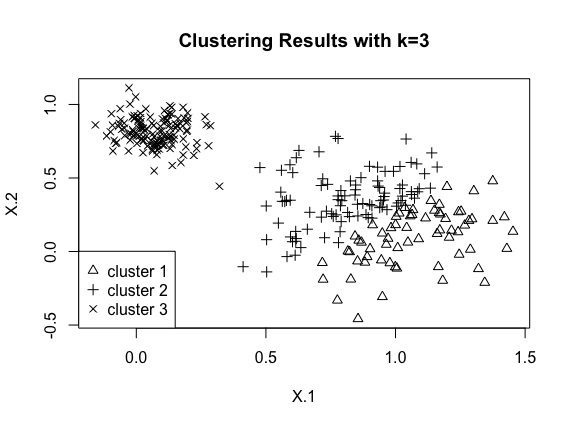
\includegraphics[width = 0.8\textwidth]{easy-3-cluster.png}
		\caption{Clustering Results with $k=3$}
		\label{fig:easy-3-cluster}
		\end{figure}

		With $k = 3$, the SSE of each cluster, the overall SSE and SSB is shown in Table \ref{tbl:sse-easy-3}

		\begin{table}[H]
		\centering
			\begin{tabular}{|c|c|c|c|c|c|c|}
			\hline
			& 1 & 2& 3& overall & overall(k=2)& overall(true) \\
			\hline
			\hline
			SSE & 1.178310  & 1.506164 & 15.283697 & 17.96817 & 19.358 & 13.694\\
			\hline
			SSB & - & - & - & 79.1544 & 78.08 & 77.76 \\
			\hline
			\end{tabular}
			\caption{SSE for Dataset 1 Clustering with $k=3$}
			\label{tbl:sse-easy-3}
		\end{table}

		The tabulation matrix is shown in Table \ref{tbl:cross-easy-3}

		\begin{table}[H]
		\centering
			\begin{tabular}{|c|c|c|}
			\hline
			& true cluster 1 & true cluster 2 \\
			\hline
			cluster 1 & 91 &  0 \\
			\hline
            cluster 2 & 47 &  6 \\
            \hline
            cluster 3 &  0 &156 \\
			 \hline
			\end{tabular}
			\caption{Cross tabulation Matrix on Dataset 1 with $k=3$}
			\label{tbl:cross-easy-3}
		\end{table}

		From Table \ref{tbl:sse-easy-3} and Table \ref{tbl:cross-easy-3} we can learn that, with $k$ increasing from 2 to 3, the overall SSE decreases, which means the clusters are more tighly clustered, on average, than those when $k=2$. While when $k=3$, SSB increases, indicating that the clusters are better seperated than $k=2$.

		\subsubsection{Dataset 2}
		When changing $k$ to$k=3$, the clustering reults for dataset 2 is as shown in Figure \ref{fig:hard-3-cluster}.

		\begin{figure}[H]
		\centering
		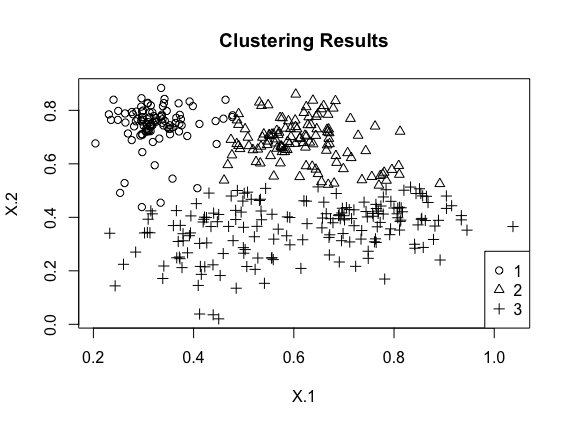
\includegraphics[width = 0.8\textwidth]{hard-cluster-3.png}
		\caption{Clustering Results with $k=3$}
		\label{fig:hard-3-cluster}
		\end{figure}

		With $k = 3$, the SSE of each cluster, the overall SSE and SSB is shown in Table \ref{tbl:sse-hard-3}

		\begin{table}[H]
		\centering
			\begin{tabular}{|c|c|c|c|c|c|c|}
			\hline
			& 1 & 2& 3& overall & overall(k=4)& overall(true) \\
			\hline
			\hline
			SSE & 0.8703093 & 1.6672667 & 7.8555954 & 10.393 & 5.556 & 4.892\\
			\hline
			SSB & - & - & - & 18.91117 & 24.41224 & 23.74813\\
			\hline
			\end{tabular}
			\caption{SSE for Dataset 1 Clustering with $k=3$}
			\label{tbl:sse-hard-3}
		\end{table}

		The tabulation matrix is shown in Table \ref{tbl:cross-hard-3}

		\begin{table}[H]
		\centering
			\begin{tabular}{|c|c|c|c|c|}
			\hline
			& true cluster 1 & true cluster 2 & true cluster 3 & true cluster 4\\
			\hline
			cluster 1& 89 &  4 &  8 &  0 \\
			\hline
            cluster 2&  0 & 96 &  3 & 17 \\
            \hline
            cluster 3&  0 &  0 & 86 & 97 \\
            \hline
			\end{tabular}
			\caption{Cross tabulation Matrix on Dataset 1 with $k=3$}
			\label{tbl:cross-hard-3}
		\end{table}

		From Table \ref{tbl:sse-hard-3} and Table \ref{tbl:cross-hard-3} we can learn that, with $k$ decreasing from 4 to 3, the overall SSE increases, which means the clusters are less tighly clustered than those when $k=4$. While when $k=3$, SSB decreases, indicating that the clusters are not so well-seperated as when $k=4$.
		
\section{Results and Analysis on the Wine dataset}
	\subsection{Clustering with Different k values}
		According to the quality attribute in the wine dataset, which varies from 3 to 8, I vary the value of $k$ from 2 to 9 while clustering the wine dataset. For each different value of $k$, I calculated the overall SSE and SSB to see which $k$ performs better on this dataset.

		The results are shown in Table \ref{tbl:wine-sse-ssb}.

		\begin{table}[H]
		\centering
			\begin{tabular}{|c|c|c|c|c|c|c|c|c|}
			\hline
			& k = 2 &  k = 3 & k = 4 &  k = 5 &  k = 6 &  k = 7 &  k = 8 &  k = 9 \\
			\hline
			SSE & 14321.978 & 12674.973 & 11452.660 & 10149.023  & 9427.378  & 8960.251  & 8307.952 & 8149.213 \\
			\hline
			SSB & 3256.022 &4903.027 &6125.340 &7428.977 &8150.622 &8617.749 &9270.048 &9428.787 \\
			\hline
			\end{tabular}
			\caption{SSE and SSB with Different $k$ Values}
			\label{tbl:wine-sse-ssb}
		\end{table}

		To show the trends clearly, I plotted Figure \ref{fig:wine-sse} and Figure \ref{fig:wine-ssb}.

		\begin{figure}[H]
		\centering
			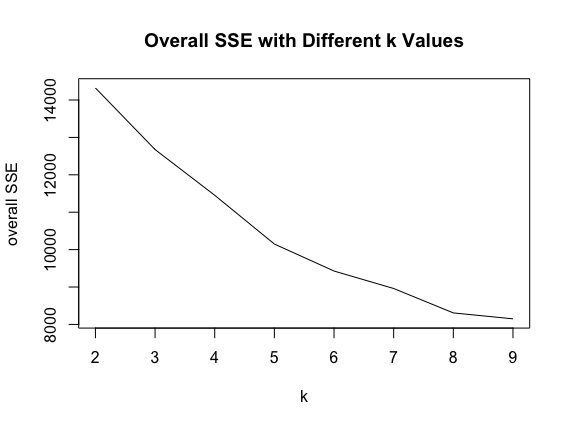
\includegraphics[width = 0.6\textwidth]{wine-sse.png}
			\caption{}
			\label{fig:wine-sse}
		\end{figure}

		\begin{figure}[H]
		\centering
			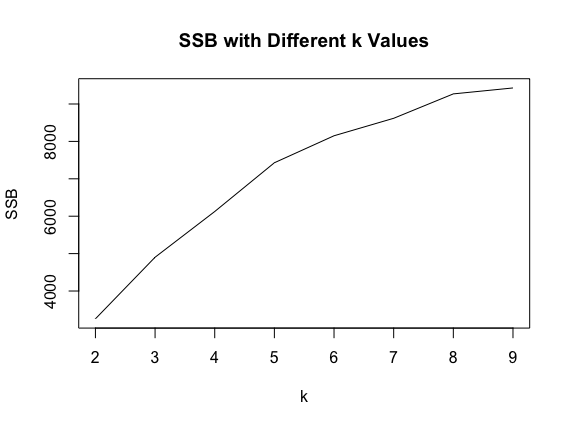
\includegraphics[width = 0.6\textwidth]{wine-ssb.png}
			\caption{}
			\label{fig:wine-ssb}
		\end{figure}

		Since SSE measures the cluster cohesion and SSB measures the cluster sepreation, we would always like to choose a k which gives relatively low SSE and high SSB. According to Figure  \ref{fig:wine-sse} and Figure \ref{fig:wine-ssb}, when k = 9, the SSE is lowest and meanwhile the SSB is highest. So I would choose $k = 9$ for the wine dataset to do clustering.

	\subsection{Clutser Validation with External Attribute}
		Since there are 6 different values for the quality attribute on wine, in this part I choose $k=6$. However, as it's hard to relabel the clusters to make them agree to the true cluster label, the cross tabulation matrix (Table \ref{tbl:wine-cross}) is not as clear as those of the two-dimensional datasets. 

		\begin{table}
		\centering
			\begin{tabular}{|c|c|c|c|c|c|c|}
			\hline
			&	quality 3&	quality 4	&quality 5	&quality 6&	quality 7&	quality 8\\
			\hline
			cluster 1&	0&	2	&25	&124	&88&	9\\
			\hline
			cluster 2&	7&	30&	288	&178	&20&	0\\
			\hline
			cluster 3&	1&	6	&229 &	95	&11&	0\\
			\hline
			cluster 4&	2&	4	&83	&126	&54&	5\\
			\hline
			cluster 5&	0&	10&	37	&106	&25&	4\\
			\hline
			cluster 6&	0&	1	&19	&9&	1&	0 \\
			\hline
			\end{tabular}
			\caption{Cross Tabulation Matrix with Quality Attribute}
			\label{tbl:wine-cross}
		\end{table}

		The reason for this non-cleararity may come from the biased data. If looking into the wine dataset, a important discovery would be that, 75\% of the records are of quality 5 or 6. So it's difficult for the data points which are not among quality 5 or 6 to cluster with k-means clustering algorithm. Meanwhile, this data is a 11-dimensional dataset. Such a high dimensionality considerably sparse the data, which also makes it difficult for k-means, which tends to form sepherical clusters.

\section{Off-the-Shelf Clutering Method}
	In this section, I used the kmeans in Weka to run on the three datasets. 
	\subsection{Dataset 1}
		For dataset 1, when $k=2$, the kmeans function gives identical results with my method.
	\subsection{Dataset 2}
		For dataset 2, when $k=4$, my method outperforms the Weka on SSE and SSB, which are shown in Table \ref{tbl:off-shelf-2}.
		\begin{table}[H]
		\centering
			\begin{tabular}{|c|c|c|}
				\hline
				& Yiran & Weka \\
				\hline
				SSE & 5.556 & 6.779 \\
				\hline
				SSB & 24.412 & 11.106 \\
				\hline
			\end{tabular}
			\caption{Comparison with Weka on Dataset 2}
			\label{tbl:off-shelf-2}
		\end{table}

	\subsection{Wine Dataset}
		For the wine dataset, Weka performs better than my method, as shown in Table \ref{tbl:off-shelf-wine}

		\begin{table}[H]
		\centering
			\begin{tabular}{|c|c|c|}
				\hline
				& Yiran & Weka \\
				\hline
				SSE & 9427.378 & 158.78 \\
				\hline
				SSB & 8150.622 & 9123.09 \\
				\hline
			\end{tabular}
			\caption{Comparison with Weka on Wine Dataset}
			\label{tbl:off-shelf-wine}
		\end{table}


\end{document}